% arara: pdflatex: { synctex: yes }
% arara: makeindex: { style: ctuthesis }
% arara: bibtex

% The class takes all the key=value arguments that \ctusetup does,
% and a couple more: draft and oneside
\documentclass[twoside]{ctuthesis}
\usepackage{float}
\usepackage{subcaption}
\usepackage{xcolor}
\usepackage{listings}
\definecolor{codegreen}{rgb}{0,0.6,0}
\definecolor{codegray}{rgb}{0.5,0.5,0.5}
\definecolor{codepurple}{rgb}{0.58,0,0.82}
\definecolor{backcolour}{rgb}{0.95,0.95,0.92}

\lstdefinestyle{mystyle}{
  backgroundcolor=\color{backcolour}, commentstyle=\color{codegreen},
  keywordstyle=\color{magenta},
  numberstyle=\tiny\color{codegray},
  stringstyle=\color{codepurple},
  basicstyle=\ttfamily\footnotesize,
  breakatwhitespace=false,         
  breaklines=true,                 
  captionpos=b,                    
  keepspaces=true,                 
  numbers=left,                    
  numbersep=5pt,                  
  showspaces=false,                
  showstringspaces=false,
  showtabs=false,                  
  tabsize=2
}
\lstset{style=mystyle}

\ctusetup{
	preprint = \ctuverlog,
%	mainlanguage = english,
%	titlelanguage = czech,
	mainlanguage = czech,
	otherlanguages = {slovak,english},
	title-czech = {Přenos telemetrických dat z meteorologického balónu},
	title-english = {Telemetric Data Transmission from Meteorological Balloon},
	subtitle-czech = {},
	subtitle-english = {},
	doctype = B,
	faculty = F3,
	department-czech = {Katedra elektromagnetického pole},
	department-english = {Department of electromagnetic field},
	author = {Jakub Dvořák},
	supervisor = {Ing. Tomáš Kořínek, Ph.D.},
	supervisor-address = {Technická 2, \\ Praha 6},
	supervisor-specialist = {},
	fieldofstudy-english = {},
	subfieldofstudy-english = {},
	fieldofstudy-czech = {},
	subfieldofstudy-czech = {},
	keywords-czech = {slovo, klíč},
	keywords-english = {word, key},
	day = 20,
	month = 5,
	year = 2022,
	specification-file = {zav_prace.pdf},
%	front-specification = true,
%	front-list-of-figures = false,
%	front-list-of-tables = false,
%	monochrome = true,
%	layout-short = true,
}

\ctuprocess

\addto\ctucaptionsczech{%
	\def\supervisorname{Vedoucí}%
	\def\subfieldofstudyname{Studijní program}%
}

\ctutemplateset{maketitle twocolumn default}{
	\begin{twocolumnfrontmatterpage}
		\ctutemplate{twocolumn.thanks}
		\ctutemplate{twocolumn.declaration}
		\ctutemplate{twocolumn.abstract.in.titlelanguage}
		\ctutemplate{twocolumn.abstract.in.secondlanguage}
		\ctutemplate{twocolumn.tableofcontents}
		\ctutemplate{twocolumn.listoffigures}
	\end{twocolumnfrontmatterpage}
}

% Theorem declarations, this is the reasonable default, anybody can do what they wish.
% If you prefer theorems in italics rather than slanted, use \theoremstyle{plainit}
\theoremstyle{plain}
\newtheorem{theorem}{Theorem}[chapter]
\newtheorem{corollary}[theorem]{Corollary}
\newtheorem{lemma}[theorem]{Lemma}
\newtheorem{proposition}[theorem]{Proposition}

\theoremstyle{definition}
\newtheorem{definition}[theorem]{Definition}
\newtheorem{example}[theorem]{Example}
\newtheorem{conjecture}[theorem]{Conjecture}

\theoremstyle{note}
\newtheorem*{remark*}{Remark}
\newtheorem{remark}[theorem]{Remark}

\setlength{\parskip}{5ex plus 0.2ex minus 0.2ex}

% Abstract in Czech
\begin{abstract-czech}
Aaaabstrakt

\end{abstract-czech}

% Abstract in English
\begin{abstract-english}
Abstract
	
\end{abstract-english}

% Acknowledgements / Poděkování
\begin{thanks}
Děkuji vedoucímu Tomáši Kořínkovi za cenné rady a pomoc při realizaci práce. Děkuji Ing. Martinu Motlovi za pomoc s vypouštěním sondy. (tmobile tracker)

\end{thanks}

% Declaration / Prohlášení
\begin{declaration}
	Prohlašuji, že jsem tuto práci vypracoval samostatně s~použitím literárních pramenů a~informací, které cituji a~uvádím v~seznamu použité literatury a~zdrojů informací.

V Praze, \ctufield{day}.~\monthinlanguage{title}~\ctufield{year}
\end{declaration}

% Only for testing purposes
\listfiles
\usepackage[pagewise]{lineno}
\usepackage{lipsum,blindtext}
\usepackage{mathrsfs} % provides \mathscr used in the ridiculous examples

\begin{document}

\maketitle

\chapter{Úvod}
tato práce ze zabývá... ano zabývá se...



\chapter{Cíl práce}
%výroba sondy schopná měřit podmínky ve tropo a posílat je na zem, měření příchozího signálu na zemi, vyrobit model šíření, změřit refrakci paprsku

	\section{Šíření vln ve troposféře}
	jak to funguje, na čem to závisí (přečíst literaturu)

	\section{Způsob řešení / návrh experimentu}
	výroba sondy, vypuštění spolu s čhmú, naměření dat z tropo a naměření dat na zemi a kombinace do modelu šíření vlny, anténa na trackeru, zjištění směrové charakteristiky, napočítat výkonovou bilanci -> výkon pro vysílání.
		\subsection{Měřená data}	
		jaká data budou měřena - podle literatury

	\section{Součásti experimentu}
	co je potřeba udělat - hw, firmware, sw, mechaniku, naměření dat, naměření charakteristik antény, zpracování dat. 


\chapter{Návrh systému}

	\section{Požadavky}
	Hlavním požadavkem je posílání telemetrických údajů o poloze a ukládání zbylých naměřených dat na SD kartu umístěnou na palubě sondy. S ohledem na panující podmínky ve vyšších vrstvách zemské atmosféry musela být sonda schopna operovat za nízkého tlaku a teploty, které panují ve vyšších vrstvách atmosféry. Toto se vztahuje jak na mikročipy a senzory, tak na baterie, používané k napájení sondy. Další podmínkou bylo spolehlivé fungování v oblasti vysoké vlhkosti - oblačnosti a za deště. 

	Z důvodu dlouhé čekací doby na povolení vypuštění balónu, které vydává Úřad pro civilní letectví, je využito povolení, které má dlouhodobě sjednané ČHMÚ. Toto povolení se vztahuje na vypouštění volných balónů s užitečným zatížením do celkové hmotnosti 600~g. Denní sonda Vaisala RS41, kterou ČHMÚ posílá 3$\times$ denně, váží 84~g. Sonda vyvíjená v rámci této práce tedy musí splňovat požadavek na hmotnost do 516~g.

	Značná část GPS přijímačů je od výrobce zablokována pro použití ve výškách větších jak 10 km n. m. a je nutné zvolit přijímač, který dovoluje tzv. \textit{airborne mode}, ve kterém není omezena pracovní výška.

	Mechanická zástavba celé sondy musí splňovat požadavky pracovníků ČHMÚ, aby nedošlo k poničeni balónu a způsobení škod při dopadu na zem. Jelikož je sonda Vaisala RS41 pověšena pod sondu vznikající v rámci této práce, je nutné zajistit robustnost a zamezit odpojení sondy Vaisala, nebo rozpadu vyvíjené sondy.


	
	\section{Elektronika sondy}
	%součástky do -40, nízký tlak (bez elektrolytických kond.), dosah 40+ km
	
	
		\subsection{Sledování sondy}
		Sledování sondy lze realizovat několika způsoby. Níže jsou popsány nejčastější z nich a jsou diskutovány výhody, nevýhody a možná rizika.

			\subsubsection{GSM tracker}
			Amatéry často využívána, nicméně velmi nedoporučovaná~\url{https://www.highaltitudescience.com/pages/tracking-a-weather-balloon} metoda je zasílání dat skrze mobilní sítě. GSM sítě, přes které se data posílají, jsou aktivní přibližně do výšky 10\,km (odkaz), není tudíž možné sledovat sondu po celou dobu letu. Velké množství sond také přistane v~neobydlených a~odlehlých oblastech, ve kterých nemusí být dostatečný signál pro přenos dat.


			\subsubsection{APRS}
			APRS (\textit{\textbf{A}utomatic \textbf{P}acket \textbf{R}eporting \textbf{S}ystem}) je radioamatéry často využívaný způsob sledování sondy, jelikož jde o~způsob levný a spolehlivý a~mnoho radioamatérů má vlastní vybavení pro posílání dat přes APRS. Základem je APRS vysílač, který lze koupit, nebo postavit. GPS data, spolu například s~teplotou a~tlakem, jsou následně takto vysílána a~přijímána amatérskými rádii~\url{https://www.highaltitudescience.com/pages/tracking-a-weather-balloon}. Data se poté buď pošlou dál, nebo se nahrají na internetovou stránku k tomuto účelu zřízenou (\url{aprs.fi}), odkud je může každý sledovat.
			Nevýhodou APRS sledovače je bohužel fakt, že pokud sonda přistane v~neobydlené a~odlehlé oblasti, kde nejsou žádné amatérské rádiové stanice, není možno data odeslat. Proto je APRS sledovač vhodný pouze jako záloha, nebo doplnění, není dobré na něj spoléhat se stoprocentní jistotou. Pokud se vysílači nepovede vyslat souřadnice místa dopadu, můžeme přesto APRS vysílač najít pomocí radiového přijímače, naladěného na vysílací frekvenci, a~směrové antény. Další nevýhoda je potřebná licence pro vysílání na frekvenci 144,8~MHz, na které probíhá APRS \url{https://www.zakonyprolidi.cz/cs/2005-156#cast1}


			\subsubsection{Satelitní sledovač}
			Další způsob je využité satelitního sledovače. Jedná se zpravidla o zařízení na sledování majetku v případě odcizení. Získaná data o~poloze se posílají přes síť satelitů na nízké oběžné dráze Země. Využívána je služba \textit{Globalstar}, jež se specializuje na provoz satelitních telefonů. Ze satelitů jsou následně data poslána na speciální internetovou stránku, kde jsou přístupná například z~počítače, nebo mobilní aplikace. Pozice lze také zaslat přes SMS bránu, jako zprávu na mobilní telefon. Výhodou je širší pokrytí oproti GSM síti. 

			Toto řešení má nicméně i~své nevýhody. GPS čip ve sledovači je omezený do maximální výšky 6\,500\,m\,n.\,m.~\url{{https://www.findmespot.com/downloads/SPOT_TRACE_User_Guide.pdf}}. Kvůli tomu nastane po dosažení takové výšky tzv. blackout, kdy GPS čip přestane reagovat. Po následném sestupu sondy pod hladinu 6\,500\,m\,n.\,m. se GPS čip opět připojí a~sledovač opět začne fungovat. Další z~problémů je fakt, že sledovač musí mít GPS anténu neustále nasměrovanou k~obloze, tudíž, pokud se při dopadu sonda nějak překlopí, není možné zaměřit její pozici.

			\subsection{Přímé posílání GPS dat}
			Pro tuto práci je implementačně nejjednodušším řešením přímé posílání GPS dat. S ohledem na zadání je nutné v rámci práce telemetrická data o poloze ze sondy posílat a tedy tyto informace lze využít k samotné lokalizaci a následnému nalezení sondy. Rizikem je dopad do oblasti, kde se omezí dosah telemetrického signálu. Např. do hustého lesa, nebo do zástavby.

			S ohledem na hmotnost, kterou by předešlá řešení přidala k celkové hmotnosti, bylo zvoleno tohoto způsobu sledování.

			\subsection{Zjištění pozice sondy ČHMÚ}
			Jak již bylo zmíněno, sonda ČHMÚ je při letu zavěšena pod vyvíjenou sondou. Data vysílaná sondou ČHMÚ jsou přijímána a dekódována v místě vypuštění, ale také jsou zachytávána amatérskými rádii a informace o poloze jsou sdílena na internetu. Tento způsob je spolehlivý, jelikož vysílací část je komerčně prodávaná a určena pro profesionální použití. Přijímacích stanic je velké množství a tedy je vysoká pravděpodobnost, že budou data ze sondy zachycena. 

			Nevýhodou je, že sonda ČHMÚ není přímou součástí vyvíjené sondy a tedy může dojít k odtržení. Tento způsob sledování je tedy brán jako záloha.


		
	\section{Firmware sondy}
	Firmware pro mikroprocesor v sondě zajišťuje inicializaci senzorů, správné čtení dat ze senzorů, jejich zpracování. Dále je nutné načítání data z GPS modulu a jejich rozdělení na dané zprávy a bloky informací využívaných pro určení pozice v prostoru. Všechny získané informace je poté nutno sešít do zprávy poslané telemetrií na zem a uložit na externí paměť. 

	Nutnou součástí firmwaru je také ošetření chybových stavů a možných errorů, vyvolaných chybným čtením dat a nebo fyzickými podmínkami prostředí.
	%čtení ze senzorů, parsování dat, posílání na zem a na sd kartu, odolnost, měření náklonu - jak?
	

\chapter{Realizace}
Tato kapitola se zabývá samotnou realizací sondy. Popisuje cestu, kterou byla práce směřována při vývoji elektroniky a popisuje výběr jednotlivých komponent. Dále vysvětluje dílčí části firmwaru sondy a způsob, jakým byly řešeny problémy. Popisuje jak vysílací část - sondu, tak přijímací části. Jednak pozemní stanici, která formátovala data do zprávy čitelné anténním trackerem a jednak přijímací software na zobrazení pozice na mapě.

	\section{Elektronika}
	
		\subsection{Způsob realizace elektroniky}
		V samotném návrhu elektroniky sondy bylo možné zvolit jednu ze dvou cest. Níže práce popisuje výhody, nevýhody a možná rizika každé z nich. Dále zdůvodňuje cestu, která byla zvolena při řešení této práce. Zmíněny jsou jak robustnost řešení, tak možná rizika způsobené lidským faktorem a časová náročnost.

		%snadné na vývoj a odladění, snadná změna zapojení pří psaní kódu
		V dnešní době existuje veliké množství mikročipů a MEMS čipů, které lze zakoupit ve formě modulů. Jedná se zpravidla o malé deky plošných spojů osazených konkrétními čipy s minimem potřebných součástek zajišťujících správné fungování. Zpravidla se jedná o blokovací kondenzátory umístěné v bezprostřední blízkosti čipů, poskytující elektrickou energii při rázovém odběru. Moduly mají vyvedené piny mikročipů na pinové lišty nacházející se na okraji PCB. 

		V případě mikroprocesoru se jedná o vývojový kit Nucleo od firmy \textit{ST Microelectronics}. Jedná se o PCB s mikroprocesorem a minimem součástek, nutných pro správné fungování procesoru. Součástí desky je také zdroj pro napájení čipu a programátor, kterým lze do mikroprocesou nahrát firmware. Jednotlivé piny mikroprocesoru jsou vyvedeny na pinové lišty na kraji desky a slouží ke snadnému propojení s moduly. 

		Výhodou tohoto řešení ve fázi vývoje je snadná záměna zapojení modulů a rychlé odstranění chyb způsobené chybným výběrem komunikačních pinů mikroprocesoru.

		Nevýhoda tohoto řešení je malá robustnost zapojení. Komunikační cesty mezi mikroprocesorem a senzory jsou zbytečné dlouhé, jelikož jsou podřízeny umístění pinů na pinových lištách. Další nevýhodou je nemožnost ovlivnit umístění blokovacích kondenzátorů u mikroprocesoru a nebo zvýšení jejich počtu. Vývojový kit Nucelo není tvořen s ohledem na malé rozměry a velikost PCB tohoto kitu ovlivňuje celkovou velikost elektroniky sondy.


		Druhá cesta, kterou je možná se vydat při vývoji elektroniky v sondě je samostatná deska, která obsahuje jednotlivé mikročipy bez jejich modulů a separátních PCB. Díky tomu je možné minimalizovat vzdálenost mezi mikroprocesorem a senzory a zvýšit robustnost napájení čipů. Celková velikost desky je poté dána především schopnostmi návrháře. 

		Toto řešení je ale časové náročné a v případě způsobené chyby se špatně ladí. V případě zničení, nebo nefunkčnosti nějaké elektronické součástky je nutné její odpájení z desky, což může ohrozit komponenty v okolí. V případě modulů lze vyměnit modul samotný.

		Při řešení této práce byla zvolena cesta modulů. Důvodem bylo malé množství času neumožňující případné zdlouhavé odlaďování zapojení a také nedostatek součástek samotných. V tomto případě byly dostupnější senzory ve formě modulů a mikroprocesor ve formě vývojového kitu. 

		\subsection{Použité komponenty}
		Níže jsou zmíněny druhy čidel, které jsou nutné pro měření podmínek v troposféře, které ovlivňují přenos radiového signálu. Jak již bylo zmíněno, senzory musí být schopny měřit veličiny v rozsahu hodnot, které panují ve troposféře. Velký výběr modulů s mnohými senzory a dalšími elektrickými součástkami nabízí firma \textit{Microelektronika}. Jená se o produky využívané pro výuku a rychlý vývoj. Výhodou je jejich sjednocený pinout a stejné rozměry konektoru (pinové lišty).

		\subsubsection{GPS modul}
		GPS moduly jsou zpravidla omezeny dvěma parametry. Maximální nadmořsou výškou 18~km a maximální rychlostí 515~m/s vůči zemi https://www.ecfr.gov/current/title-22/part-121. Někteří výrobci GPS modulů berou tato omezení v konjunkci, kdy pro zablokování modulu musí platit obě podmínky, někteří výrobci uvažují  disjunkci, kdy stačí, aby nastala jedna z pomínek a modul přestane dávat validní data. Modul, který byl vybrán je u-blox SAM-M8Q. Podle dokumentace GPS modulu (\url{https://www.u-blox.com/sites/default/files/SAM-M8Q_DataSheet_%28UBX-16012619%29.pdf}) je maximální výška 50~km a maximální rychlost 500~m/s. V případě letu balónu nebude splněna ani jedna z podmínek. Tento GPS modul je součástí vývojového modulu GNSS 4 Click od firmy \textit{Microelektronika}.

		U-blox moduly nabízí široké množství pracovních módů podle charakter použití. Pro běžné použití se využívá mód \textit{Portable}. Jedná se o kompromis mezi rozsahem a přesností určení pozice. Další módy jsou zobrazeny v tabulce \ref{tab:ublox:modes}. V případě sondy byl zvolen mód Airborne \textless{}1g. Při letu sondy není očekáváno zrychlení přesahující 1~g a rychlosti nad 100~m/s (360~km/h). 
		\begin{table}[]
			\centering
			\caption{Módy GPS přijímačů u-blox}
			\label{tab:ublox:modes}
			\begin{tabular}{|l|c|c|c|c|}
				\hline
				Platform &
				Max Altitude{[}m{]} &
				\begin{tabular}[c]{@{}c@{}}MAX Horizontal\\ Velocity {[}m/s{]}\end{tabular} &
				\begin{tabular}[c]{@{}c@{}}MAX Vertical\\ Velocity {[}m/s{]}\end{tabular} &
				\begin{tabular}[c]{@{}c@{}}Max Position \\ Deviation\end{tabular} \\\hline
				Portable               	& 12000 & 310 & 50  & Medium \\\hline
				Stationary             	& 9000  & 10  & 6   & Small  \\\hline
				Pedestrian             	& 9000  & 30  & 20  & Small  \\\hline
				Automotive             	& 6000  & 84  & 15  & Medium \\\hline
				At sea                 	& 500   & 25  & 5   & Medium \\\hline
				Airborne \textless{}1g 	& 50000 & 100 & 100 & Large  \\\hline
				Airborne \textless{}2g 	& 50000 & 250 & 100 & Large  \\\hline
				Airborne \textless{}4g 	& 50000 & 500 & 100 & Large  \\\hline
				\end{tabular}
			\end{table}
		
		\subsubsection{Teplotní a tlakový senzor}
		Podle (\url{https://www.sensorsone.com/altitude-pressure-units-conversion/}) se tlak ve výšce 30~km pohybuje kolem hodnoty 10~mbar. S ohledem na očekávané rozsahy měřeného tlaku a teploty byl vybrán senzor MS5607 od firmy \textit{TE Connectivity}. Rozsahy měřitelných hodnot jsou zaneseny v tabulce \ref{tab:ms:range}. Teplotní a tlakový senzor je součástí modulu od firmy \textit{Parallax}. Výrobce na stránkách produktu \url{https://www.parallax.com/product/altimeter-module-ms5607/} uvádí, že senzor byl úspěšně testován ve výšce 36~km.
		
		\begin{table}[]
			\begin{tabular}{|l|lll|l|}
			\hline
			Pressure   & \multicolumn{1}{l|}{Min}  & \multicolumn{1}{l|}{Typ} & Max  & Unit \\ \hline
			Range      & \multicolumn{1}{l|}{10}   & \multicolumn{1}{l|}{}    & 1200 & mbar \\ \hline
			Range      & \multicolumn{1}{l|}{-40}  & \multicolumn{1}{l|}{}    & 85   & °C   \\ \hline
			Resolution & \multicolumn{3}{c|}{\textless{}0.01}                        & °C   \\ \hline
			Accuracy   & \multicolumn{1}{l|}{-0.8} & \multicolumn{1}{l|}{}    & 0.8  & °C   \\ \hline
			\end{tabular}
			\caption{Rozsah senzoru MS5607, převzato z \url{https://www.parallax.com/package/altimeter-module-ms5607-datasheet})}
			\label{tab:ms:range}
		\end{table}

		
		\subsubsection{Vlhkostní senzor}
		Vlhkostní senzor byl zvolen AM2320, který je součástí modulu DHT22 Click od firmy \textit{Microelektronika}. Senzor je schopen měřit v rozsahu od -40 do 80~°C a 0 až 100~\% relativní vlhkosti (\url{https://cdn-shop.adafruit.com/product-files/3721/AM2320.pdf}). 

		\subsubsection{Senzor orientace}
		Pro zjištění orientace bylo použito senzoru MPU9250, který je součástí modulu 9DOF Click. Jedná se o gyroskop Senzor resp. modul byl vybrán, jelikož byl již dříve používán na jiných projektech a byl ihned dostupný. Díky tomu bylo ihned možné přejít ke psaní ovladače pro vyčítání dat a jeho implementaci do systému. Senzor také splňuje rozsah pracovních teplot a lze tedy využít v podmínkách, které při letu nastanou (\url{https://invensense.tdk.com/wp-content/uploads/2015/02/PS-MPU-9250A-01-v1.1.pdf}).  
		
		
		
		
		\subsection{Testování elektroniky}
		měření odběru, energie pro poslání dat


		\subsection{PCB pro připojení modulů}
		%Navrženy shieldy, nakresleny modely. Spínaný zdroj + LDO, ochrany vstupů, volné GPIO na rozšíření
		Ve vývojové fázi práce byly moduly zapojeny skrze nepájivé pole a propojeny propojovacími kabely s piny Nucleo desky. Moduly byly postupně přidávány souběžně s vývojem softwaru. Po odladění komunikace se všemi použitými moduly byly vytvořeny dvě redukční PCB na propojení Nucleo kitu a modulů. Moduly jsou vyobrazeny na obr. \ref{fig:shield:top} a \ref{fig:shield:bot}. 

		\begin{figure}[hbtp]
			\centering
			\begin{subfigure}{0.3\textwidth}
				\centering
				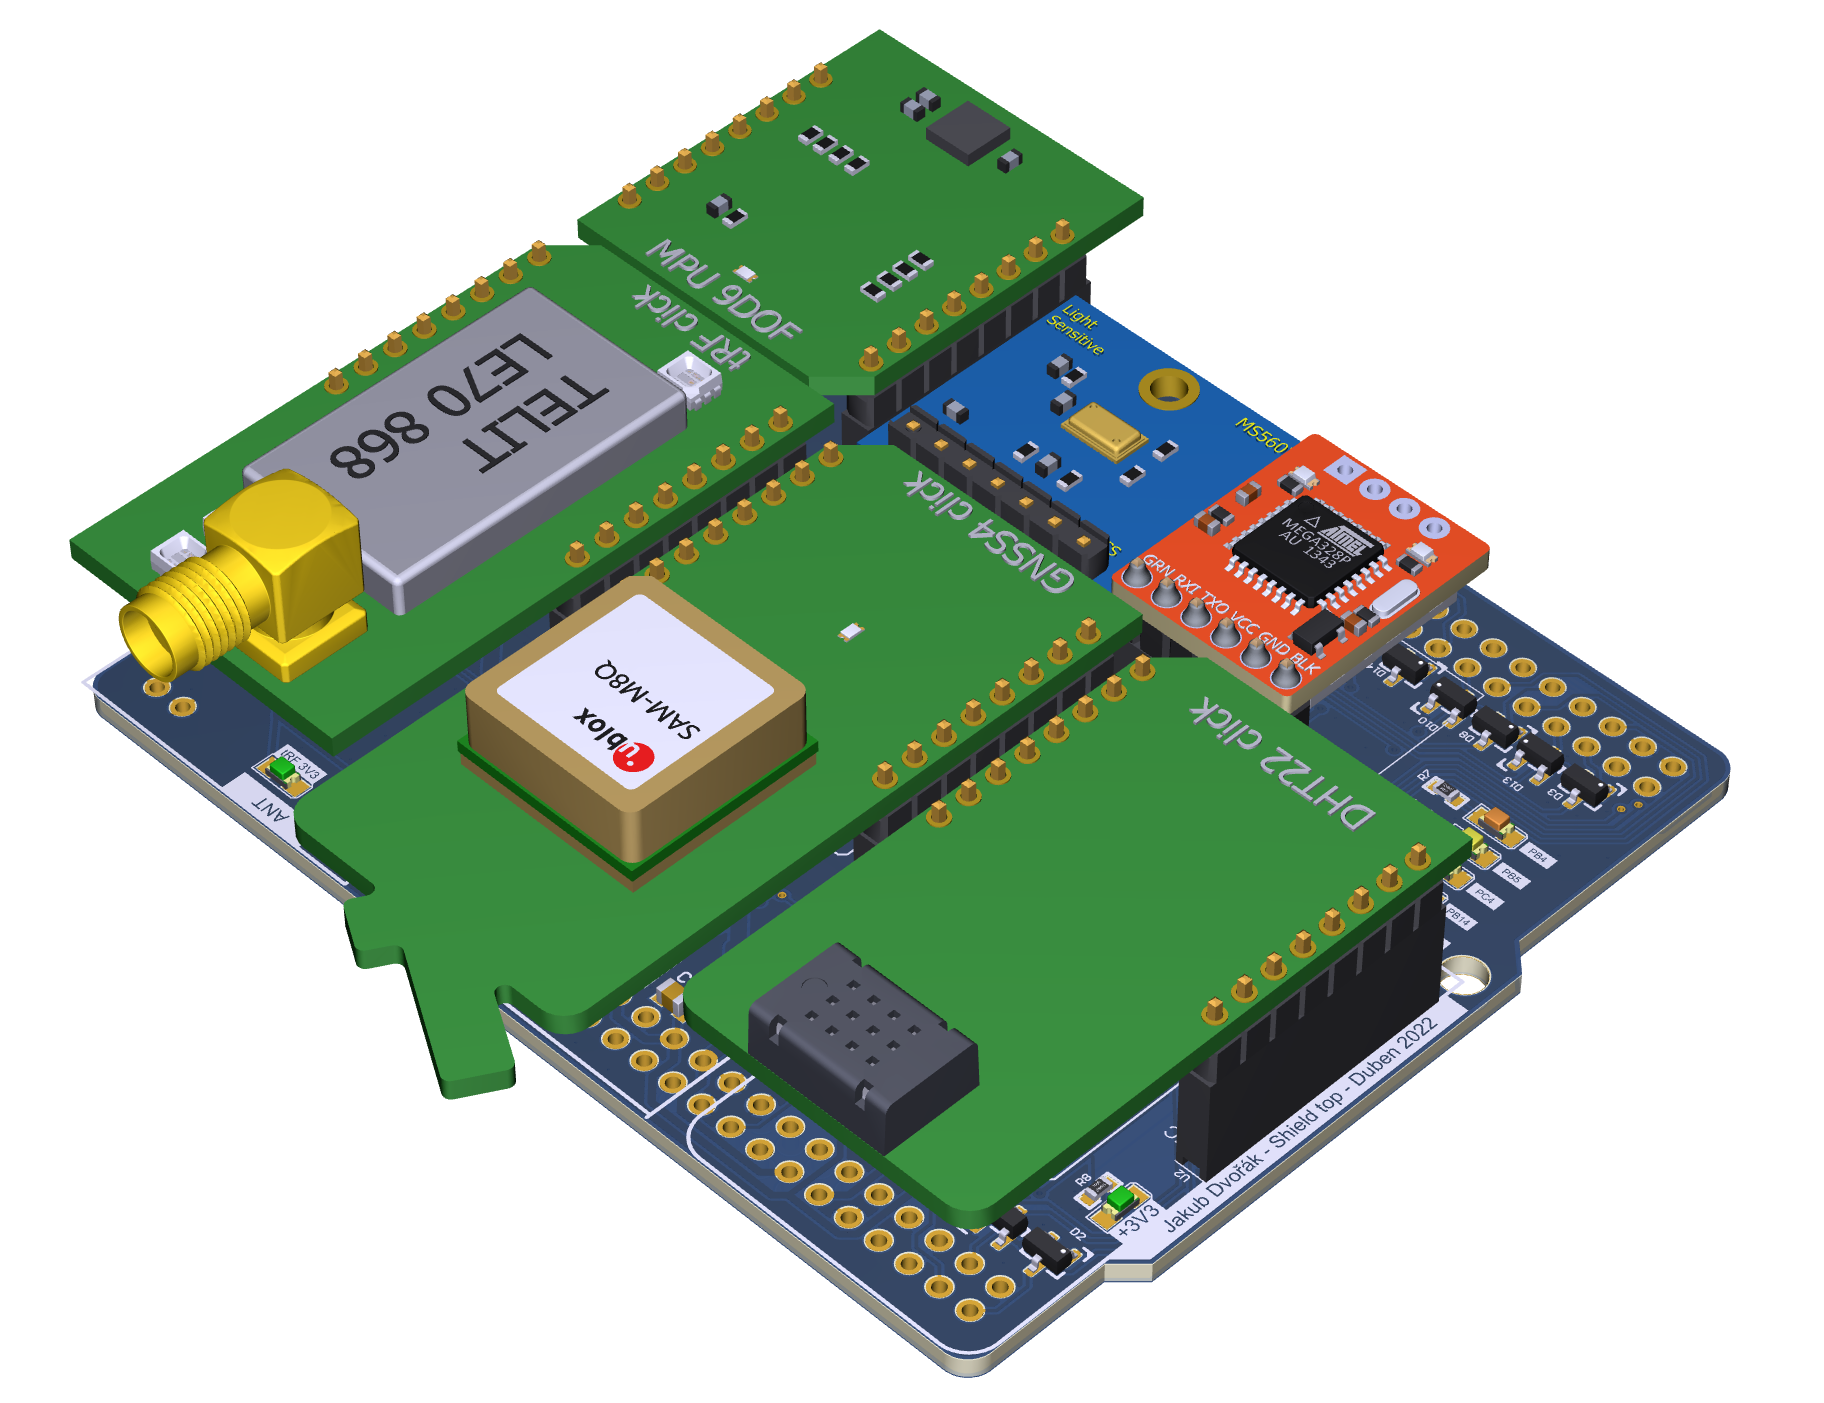
\includegraphics[height=0.7\linewidth]{Figures/shield_top.png} 
				\caption{Vrchní redukční deska}
				\label{fig:shield:top}
			\end{subfigure}%
			\begin{subfigure}{.3\textwidth}
				\centering
				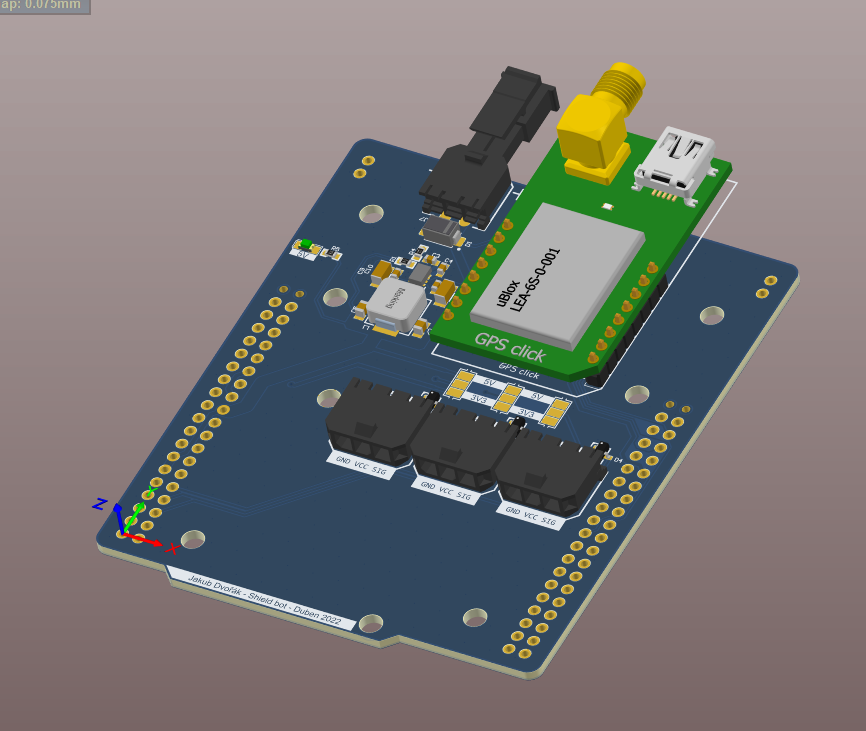
\includegraphics[height=0.7\linewidth]{Figures/shield_bot.png}
				\caption{Spodní redukční deska}
				\label{fig:shield:bot}
			\end{subfigure}
			\begin{subfigure}{.3\textwidth}
				\centering
				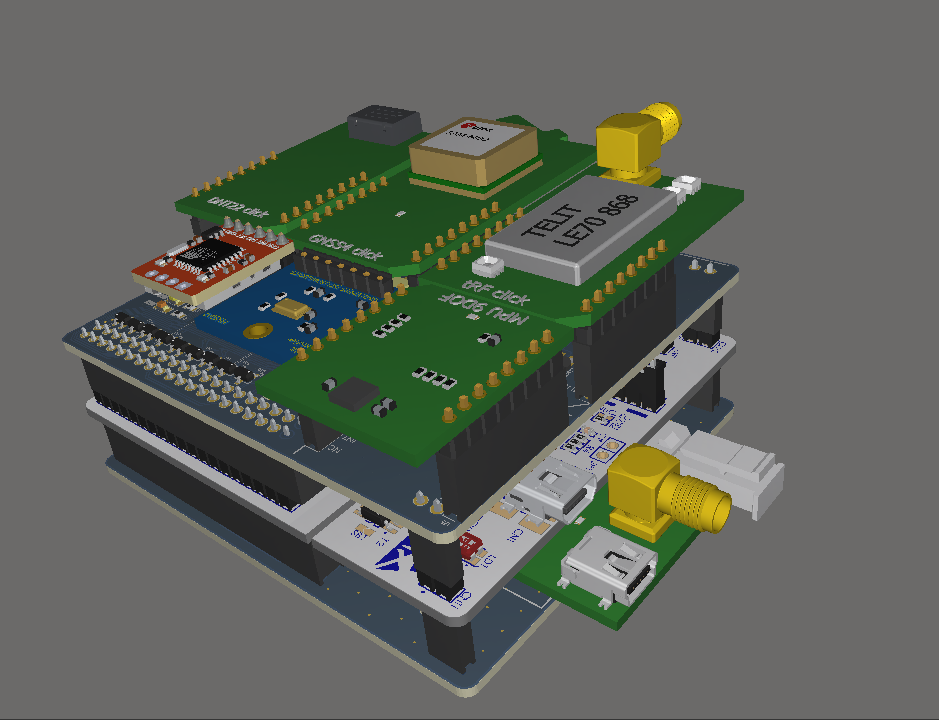
\includegraphics[height=0.7\linewidth]{Figures/shield_assembly.png}
				\caption{Sestava PCB}
				\label{fig:shield:assembly}
			\end{subfigure}
			\caption{Redukční desky pro moduly}
			\label{fig:shields:pcb}
		\end{figure}

		\subsection{Napájení}
		Jako zdroj energie po dobu letu byly vybrány tužkové baterie \textit{Energizer ultimate lithium}. Dle technického listu (\url{https://data.energizer.com/pdfs/l91.pdf}) jsou schopny operovat až do teploty -40~°C při poklesu kapacity z xxx na xxx mAh. S ohledem na teploty panující ve stratopauze, které klesají až k -60~°C, byl počet zvýšen na 10 ks, nechávající kapacitní rezervu. 

			\subsubsection{Zdroje}
			Vstupní napětí se v závislosti na teplotě a momentálním odběru pohybuje od 18~V do 10~V. Pro zvýšení účinnosti byl jako hlavní regulátor využit spínaný zdroj. S ohledem na dostupnost součástek a ověřenost funkčnosti byl vybrán spínaný zdroj \textit{LMR33630} od firmy \textit{Texas Instruments}. Účinnost tohoto zdroje se pohybuje od TODO: zjistit z DSH. 

			Další výhodou spínaného zdroje je minimální PSRR - \textit{Power Source Rejection Ratio}. Výstupní napětí zůstává konstantní bez ohledu na změnu napětí na vstupu, dokud není překročeno minimální napájecí napětí. TOTO: kolik pro 5V vout. 
			
			Nevýhodou spínaných zdrojů je zanášení šumu do obvodu. Tento problém se vyřeší využitím lineárního regulátoru. Šum generovaný spínacím regulátorem by mohl způsobit nesprávné fungování mikroprocesoru a snižovat kvalitu příjmu GPS modulu. V tomto případě byla napájecí topologie následující. Napětí baterií bylo na spodní redukční desce spínacím regulátorem sníženo na 5~V. Toto napětí bylo následně skrze nevyužité piny vývojového kitu Nucleo přivedeno na horní redukční desku, kde bylo lineárním regulátorem sníženo na 3,3~V. Celkem jsou na desce tři větve s tímto napětím. Mikrokontrolér a senzory mají vlastní větev. Další lineární regulátor napájí pouze GPS modul a třetí lineární regulátor je určen pro radiový vysílač. Díky tomu nebude docházet k poklesu napětí napájení ve zbytku přístroje při vysílání dat. 

			\begin{figure}
				\centering
				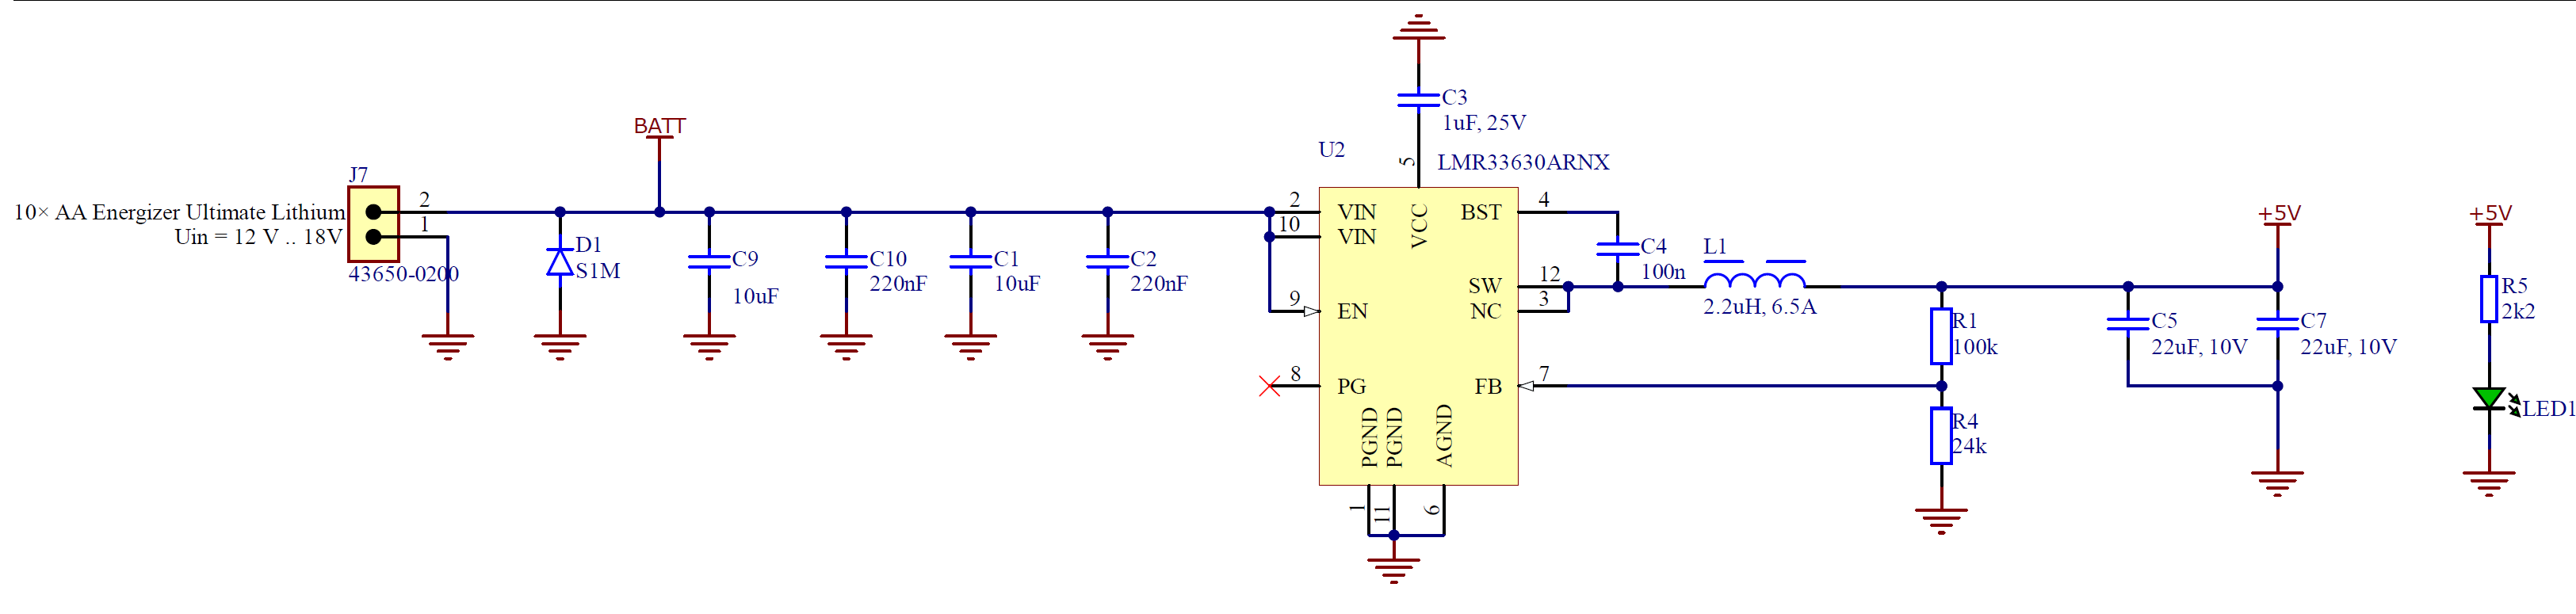
\includegraphics[width = \textwidth]{Figures/psu_bot.png}
				\caption{Schéma spínaného zdroje umístěného na spodní redukční desce}
				\label{fig:psu:bot}
			\end{figure}
			\begin{figure}
				\centering
				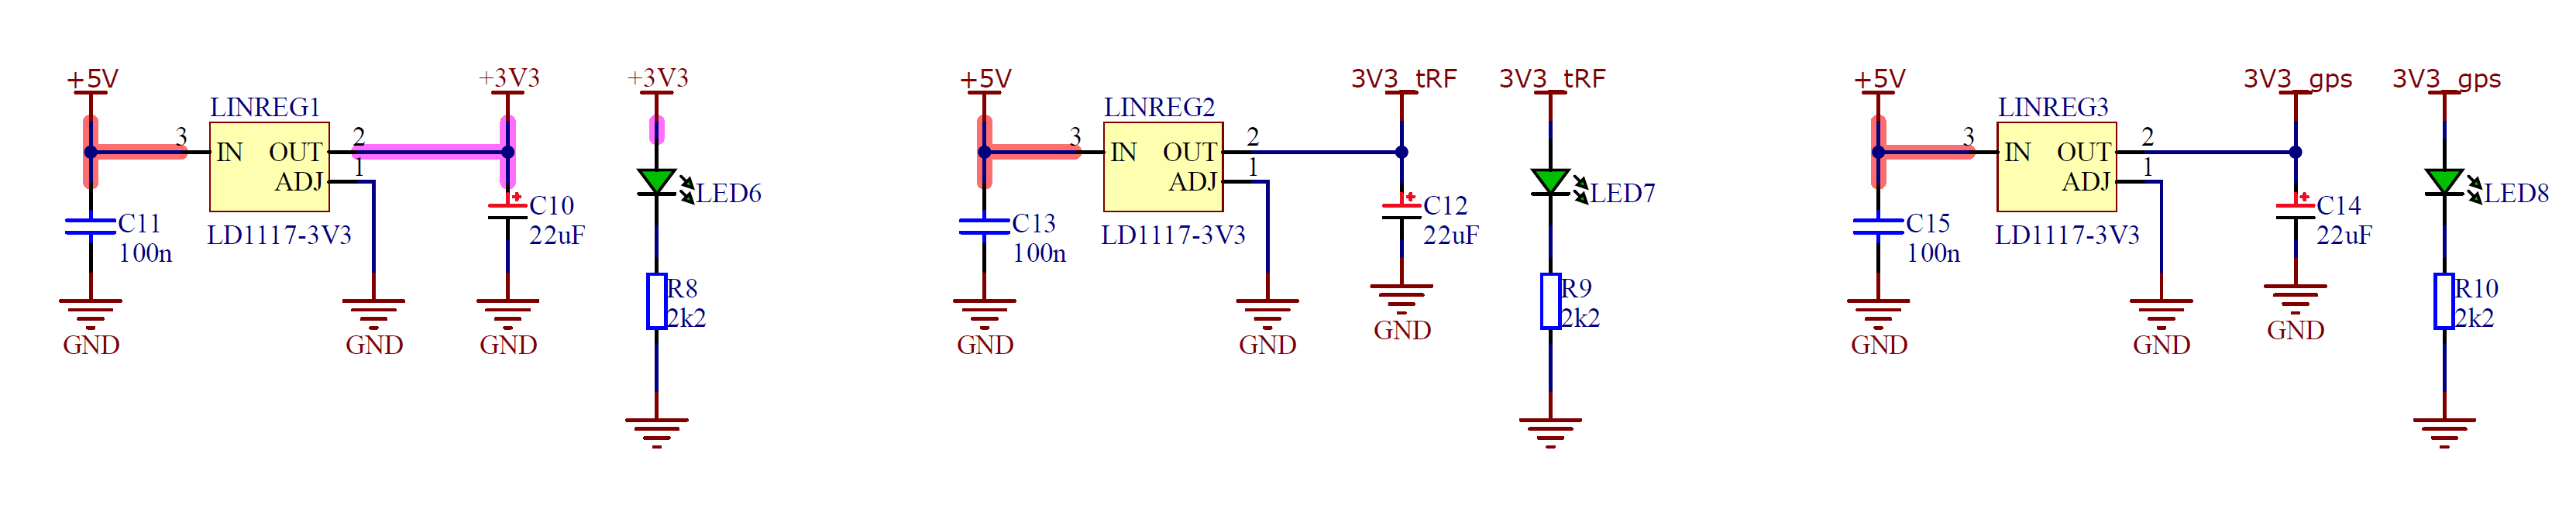
\includegraphics[width = \textwidth]{Figures/psu_top.png}
				\caption{Schéma lineárních regulátorů umístěných na horní redukční desce}
				\label{fig:psu:top}
			\end{figure}


			\subsubsection{Ochrana pinů}
			Jelikož většina pinů využívaných ke komunikaci byla snadno dostupná na dotyk při manipulaci, bylo potřeba je ošetřit vůči elektrostatickému výboji (ESD), který by měl za následek zničení čipu. Příklad ošetření GPIO pinů pomocí TVS diody BAV99 je na obr. \ref{fig:osetreni:vstupu}.
			
			\begin{figure}
				\centering
				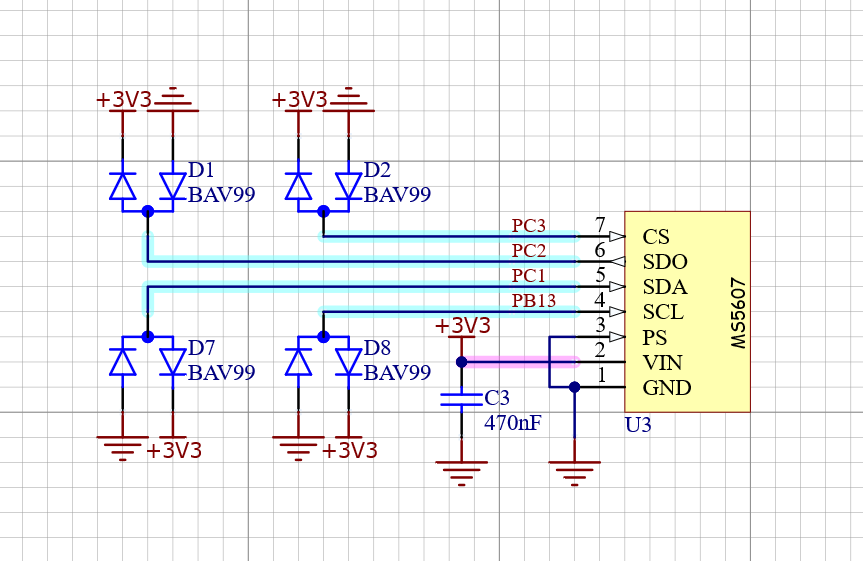
\includegraphics[width = .7\textwidth]{Figures/osetreni_vstupu.png}
				\caption{Příklad ošetření vstupů TVS diodami}
				\label{fig:osetreni:vstupu}
			\end{figure}




	\section{Mechanická zástavba}

	Součástí práce je i mechanická zástavba kryt pro elektroniku. Pro přehlednost a optimální model krytu bylo potřeba vymodelovat i jednotlivé moduly. Kolem přesného 3D modelu elektroniky mohl být vymodelován kryt bez nutnosti čekat na výrobu redukčních desek.
	\begin{figure}[hbtp]
		\centering
		\begin{subfigure}{.5\textwidth}
			\centering
			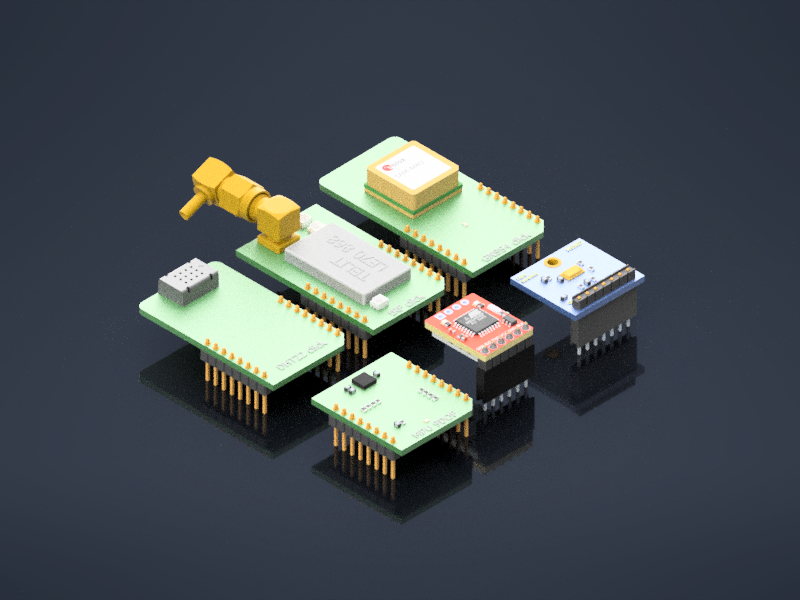
\includegraphics[height=.7\linewidth]{Figures/modules_assembly.png} 
			\caption{Vymodelované moduly}
			\label{fig:modules:assembly}
		\end{subfigure}%
		\begin{subfigure}{.5\textwidth}
			\centering
			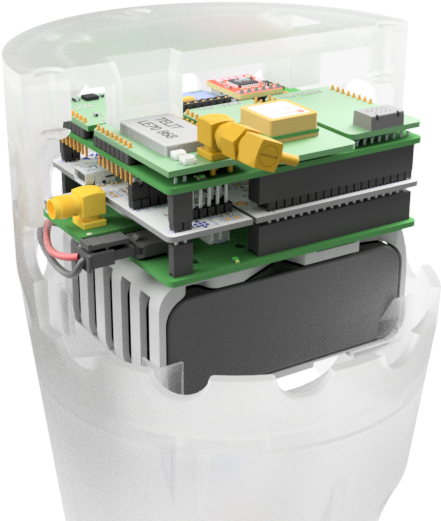
\includegraphics[height=.7\linewidth]{Figures/ALL_rez_white.png}
			\caption{Řez vrchní částí krytu sondy}
			\label{fig:all:rez}
		\end{subfigure}
		\label{fig:shields}
	\end{figure}

	
	Díky jednotlivým modelům bylo možné vytvořit kompletní model elektronické části, kolem kterého byl poté vymodelován kryt (obr. \ref{fig:all:rez}). Kryt byl modelován s ohledem na anténu umístěnou ve spodní části. Stěny kolem antény jsou ztenčené, aby co nejméně ovlivnily ladění antény na 868~MHz. Malá mechanická odolnost stěn je kompenzována čtyřmi výztužemi vedoucí po obvodu stěny.

	Pro splnění hmotnostního limitu byl model krytu postupně odlehčován. Při ubírání materiálu bylo nutné brát v potaz, že hlavní původ velké hmotnosti není při 3D tisku objem tělesa, ale jeho stěny. Při tvorbě otvorů v modelu se tedy neušetřila hmotnost odpovídající objemu válce odebraného ze stěny, ale pouze dvěma jeho podstavám. Naopak materiál byl potřeba na plášť odebraného válce.

	TODO: názorný jednoduchý model s dírou a bez, iterace 

	Připojení sondy ČHMÚ bylo provedeno pomocí gumového pásu, do kterého se zastrčila skoba odvíječe. To je zařízení, které zajistí postupné odmotání 50m lanka. 50~m je vzdálenost daná výrobcem, která musí být od balónu a dalších součástí sondy, aby byla zajištěna validní měření.

	TODO: obrázek připojení sondy

	V případě, že by došlo k delaminaci 3D tisku, byla jak elektronika, tak sonda ČHMÚ přivázána pojistným provázkem uchyceným k hlavnímu závěsu spolu s padákem a balónem. Díky tomu by sonda stále zůstala pohromadě i když by došlo k rozbití/rozlomení krytu.

	model PCB, model sondy, iterace, odlehčování, připojení sondy čhmú, bezpečnostní závěsy

	\section{Firmware}
	\subsection{Obsluha senzorů}
	Pro vyčítání dat ze senzorů bylo potřeba napsání driveru. Ten má za úkol jak vyčtení dat ze senzoru, tak jeho samotnou inicializaci a nastavení. 

	Výčet dat ze senzoru AM2320 probíhá příkazem
	\lstinputlisting[language=C]{Code/am2320_write.txt}

	Senzor následně vyšle data obsahující informace o vlhkosti a teplotě. Jejich příjem zajišťuje funkce
	\lstinputlisting[language=C]{Code/am2320_read.txt}

	Způsob přepočtu získaných dat na hodnoty teploty a tlaku je popsán v dokumentaci senzoru. Kód pro přepočet je následující:
	\lstinputlisting[language=C]{Code/am2320_get_values.txt}

	Pro senzor teploty a tlaku MS5607 je způsob výčtu dat obdobný. Nejdříve se pošle žádost o převod hodnoty jdoucí ze senzoru.
	\lstinputlisting[language=C]{Code/ms5607_convert_press.txt}
	Následně se pošle žádost o vyčtení hodnot 24bit analogově digitálního převodníku pomocí následujícího kódu.
	\lstinputlisting[language=C]{Code/ms5607_get_press.txt}

	Hodnoty změřené tímto způsobem jsou nekompenzované a jsou ovlivněny nelinearitou senzoru. Pro správnou kompenzaci teploty a tlaku je zapotřebí využít vývojový diagram na obr. \ref{fig:ms5607:flowchart}.
	\begin{figure}
		\centering
		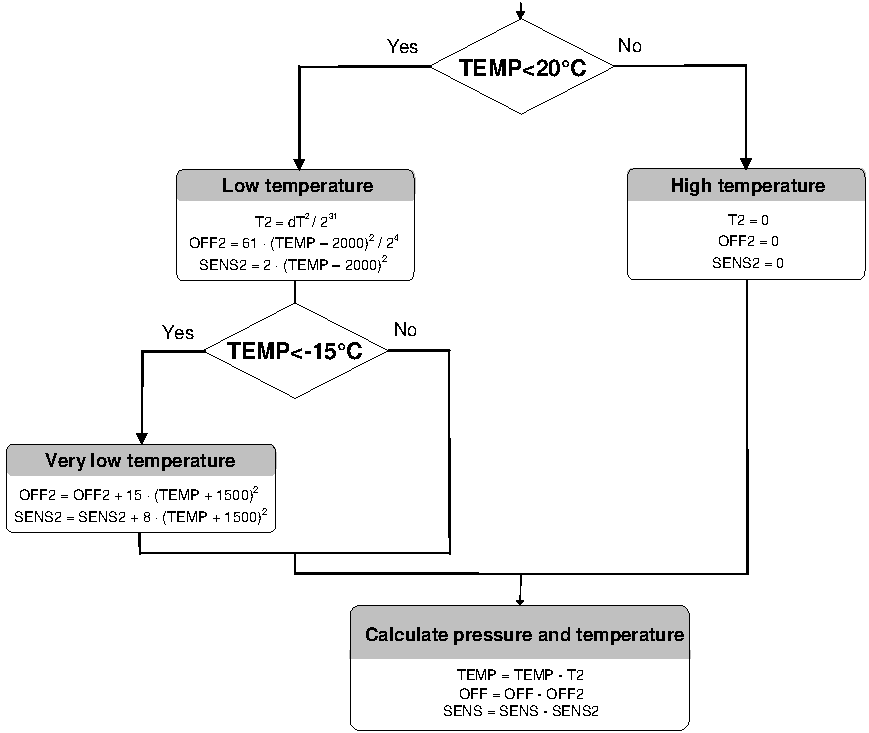
\includegraphics[width=.7\textwidth]{Figures/MS5607_flowchart.pdf}
		\caption{Vývojový diagram pro kompenzaci měřených hodnot senzorem MS5607, převzato z \url{https://www.parallax.com/package/altimeter-module-ms5607-datasheet/}}
		\label{fig:ms5607:flowchart}
	\end{figure}

	Na rozdíl od předešlých senzorů, tento senzor měří hodnoty a ukládá je do příslušných registrů průběžně. Registry senzoru jsou popsány v dokumentu \url{https://invensense.tdk.com/wp-content/uploads/2015/02/RM-MPU-9250A-00-v1.6.pdf}. Slouží k nastavení senzoru samotného, jeho identifikaci a k výčtu naměřených dat. U senzoru je potřeba nastavit vzorkovací frekvenci, rozsahy měřených hodnot a zdroj hodin. Pro následný přístup k datům na dané adrese se využije následujícího příkazu.
	\lstinputlisting[language=C]{Code/MPU_read_CMD.c}
	Senzor následně vyšle hodnoty daného registru a jejich příjem proběhne pomocí funkce níže. Hodnoty ReadAddr a READWRITE\_CMD jsou definovány v \url{https://invensense.tdk.com/wp-content/uploads/2015/02/RM-MPU-9250A-00-v1.6.pdf}.
	\lstinputlisting[language=C]{Code/MPU_read.c}
	

	\subsection{Zjištění náklonu sondy}
	TODO:
	\begin{enumerate}
		\item Obr. kyvadla a sil - nelze měřit náklon pomocí acc
  		\item Nelze měřit přes mag - vizualizace rotace kolem vektoru mag. pole
    	\item Řešení v flightcontrollerech na dronech - kalman, příliš složité na implementaci, komplementární filtr
     	\item Moje řešení
	\end{enumerate}
	


\section{Pozemní stanice}
Firmware pro mikroprocesor v pozemní stanici zodpovídá za správné dekódování přijatých telemetrických údajů. Firmware musí určit, která data jsou validní. Přijatá data je poté nutno zformátovat do zprávy určené pro anténní tracker, umístěný na střeše budovy FEL. Firmware musí být odolný vůči náhodným chybám způsobených přenosem na velkou vzdálenost. Příjem i posílání dat probíhá přes sériovou linku. 

Elektronika pozemní stanice není vystavena extrémním podmínkám a není nutné řešit její odolnost vůči vnějším vlivům. 

\section{Software pro zobrazení telemetrických údajů}
Software určený pro příjem dat na počítači umístěném v automobilu jedoucí ve směru dopadu sondy. Software musí určit validní data a vyznačit GPS pozici sondy na mapě. Další funkcí softwaru je výpis souřadnic, výšky a rychlosti sondy a teploty okolí sondy. Data jdoucí do programu jsou posílána přes sériovou linkou z přijímače signálu vysílaného sondou. 

	výstřizky kódu z driverů, sample GPS dat, vyčítání z teplota/tlak, tlak/vlhkost, gyro/acc/mag, parsovací funkce, změřené minimum accelerace v z-ose, sešití dat, watchdog, reset při erroru

	\section{Software}
	parsování příchozích dat, doplnění NMEA zprávy pro tracker, python - parsování a přepočítání souřadnic, zobrazení na mapě, zobrazení v terminálu

	\section{Testování a měření}
	Měření směrové charakteristiky proběhlo na katedře elektromagnetického pole v bezodrazné komoře. Sonda připevněna na pohyblivou osu byla otáčena motorem a byl měřen přijatý výkon anténou umístěné naproti sondě. Díky tomu byla změřena vyzařovací charakteristika antény v rozsahu 360~°C. Celkem byly měřeny 4 směrové charakteristiky a to pro různá natočení sondy kolem své osy. Směrové charakteristiky jsou zaneseny na (obr)

	TODO - graf směrových charstik.

	Dále byla měřena polarizace antény. V tomto případě byla sonda pevně umístěna na podstavci a otáčeno bylo přijímací anténou v její ose. Pro ideální kruhově polarizovanou anténu by nezáleželo na natočení přijímací antény. V případně antény umístěné v sondě je přenos znárorněn na obr. xxx.

	TODO - graf polarizace


	směrová charakteristika, teplotní odolnost v klimakomoře, proudový odběr telitu, výlet na Říp, mapa viditelnosti z bodu na mapě. 




\chapter{Experiment}
příjem dat, umístění antény na střeš e , nastavení spektráku
	\section{Průběh experimentu}
	jak to probíhalo, co se stalo, proč sonda přestala vysílat, proč doletěla jen do 17 km, nalezení pomocí sondy čhmú, sundání sondy

	\section{Naměřená data}
	co bylo na SD kartě, výsledky měření - čístě změřená data



\chapter{Výsledky}
	\section{Výstup z experimentu}
	výsledky, co bylo změřeno a zjištěno

	\section{Zpracování dat}
	zkombinovat data ze země a data ze strato, vzorečky, určit refrakci, výkonovou bilanci podle podmínek, vzít v potaz směrovou charstiku. vyrobit model šíření, grafy

	



\chapter{Závěr}
	\section{Shrnutí experimentu}
	co se povedlo, co se nepovedlo. Vyrobil jsem sondu a sw, přestala vysílat - proč? 

	\section{Možná vylepšení}
	malé pcb bez modulů, optimalizace sw, nepoužívat HAL, programovat přes registry, měření náklonu sondy, častější posílání dat, nezávislost na GPS




\appendix

\printindex

\appendix

\bibliographystyle{amsalpha}
\bibliography{ctutest}

\ctutemplate{specification.as.chapter}

\end{document}

%vaisala datasheet https://www.vaisala.com/sites/default/files/documents/WEA-MET-RS41SGP-Datasheet-B211444EN.pdf